% main.tex
%	Last update: 2019/09/05 F.Kanehori
%
\documentclass[a4j,12pt]{jsarticle}
\usepackage{dirtree}
\usepackage{setspace}
\usepackage{longtable}
%\usepackage{comment}
\usepackage[dvipdfmx]{graphicx}
\usepackage{lscape}
\usepackage{lwarp_macros}

\setlength{\textheight}{\paperheight}   % 紙面縦幅を本文領域にする(BOTTOM=-TOP)
\setlength{\topmargin}{4.6truemm}       % 上の余白を30mm(=1inch+4.6mm)に
\addtolength{\topmargin}{-\headheight}  % 
\addtolength{\topmargin}{-\headsep}     % ヘッダの分だけ本文領域を移動させる
\addtolength{\textheight}{-60truemm}    % 下の余白も30mm(BOTTOM=-TOPだから+TOP+30mm)

\setlength{\textwidth}{\paperwidth}     % 紙面横幅を本文領域にする(RIGHT=-LEFT)
\setlength{\oddsidemargin}{-0.4truemm}  % 左の余白を25mm(=1inch-0.4mm)に
\setlength{\evensidemargin}{-0.4truemm} % 
\addtolength{\textwidth}{-50truemm}     % 右の余白も25mm(RIGHT=-LEFT)

\begin{document}
% macro.tex
%	Last update: 2018/08/16 F.Kanehori

\makeatletter

%% need original symbol
\def\orgLAB{<}
\def\orgRAB{>}

%% some character usage
\catcode`\_=\active
\catcode`\^=\active
\catcode`\<=\active
\catcode`\>=\active
\def_{\ifmmode\sb\else\_\fi}
\def^{\ifmmode\sp\else\^\fi}
\def<{\ifmmode\langle\else\tt{\orgLAB}\fi}
\def>{\ifmmode\rangle\else\tt{\orgRAB}\fi}
\def\LSB{\ifmmode$[$\else\tt{[}\fi}
\def\RSB{\ifmmode$[$\else\tt{]}\fi}
\def\Ctrl#1{\tt{\,\textasciicircum#1}}
\def\BS{\tt{\symbol{'134}}}

%% alias for fonts
\let\it@\it
\let\tt@\tt
\let\bf@\bf
\let\rm@\rm
\let\gt@\gt
\let\mc@\mc
\def\it#1{{\it@{#1\,}}}
\def\tt#1{{\tt@{#1}}}
\def\bf#1{{\bf@{#1}}}
\def\rm#1{{\rm@{#1}}}
\def\gt#1{{\gt@{#1}}}
\def\mc#1{{\mc@{#1}}}
\def\Use@font#1#2{%
	\if#1t\tt{#2}\else
	\if#1i\it{#2}\else
	\if#1b\bf{#2}\else
	\if#1r\rm{#2}\else
	\if#1g\gt{#2}\else
	\if#1m\mc{#2}\else\rm{#2}\fi\fi\fi\fi\fi\fi}

%% make local scope
%
\def\LocalScope{\begingroup}
\def\endLocalScope{\endgroup}

%% dimensions
\newdimen\WID \WID=20pt		% standard indent width

%% spaces
%  \Vskip{amount}
%  \Hskip{amount}
%	amount		amount of skip (dimen)
%
\def\Vskip#1{\begin{Vmode}\vspace{#1}\end{Vmode}}
\let\Hskip\hspace

%% force vertical mode
%  \begin{Vmode} ... \end{Vmode}
%
\def\Vmode{\ifvmode\relax\else\par\hrule width 0pt height .5\baselineskip\fi}
\def\endVmode{\relax\par}

%% citation
%  \FromHere
%	...
%  \TillHere
%
\def\FromHere{%
	\\\rule{0pt}{1.8em}
	{\scriptsize{\DARROW \DARROW �������� \DARROW \DARROW}}\\}
\def\TillHere{%
	{\scriptsize{\UARROW \UARROW �����܂� \UARROW \UARROW}}\\
	\rule{0pt}{1.9em}}

%% ruler / underline
%
\def\RuleToEol#1{\hrule width \linewidth height #1}
\let\UL\underline

%% quoted word
%
\def\SQuote#1{\hspace{0pt}\Quote@{`}{#1}{'}}
\def\DQuote#1{\hspace{0pt}\Quote@{"}{#1}{"}}
\def\KQuote#1{\hspace{0pt}\Quote@knj{\,#1}}
\def\Quote@#1#2#3{\hbox{\,\raise.4ex\hbox{{\tt #1}}#2\raise.4ex\hbox{{\tt #3}}\,}}
\def\Quote@knj#1{\hbox{\,\raise.4ex\hbox{``}#1\,\raise.4ex\hbox{''}}}
\def\UpSQs{\hbox{\raise.4ex\hbox{{\tt `}}}}
\def\UpSQe{\hbox{\raise.4ex\hbox{{\tt '}}}}
\def\UpDQs{\hbox{\raise.4ex\hbox{{\tt "}}}}
\def\UpDQe{\hbox{\raise.4ex\hbox{{\tt "}}}}
\let\UpDQ\UpDQs

%% abbreviations
%
\def\RArrow{$\rightarrow$}
\def\LArrow{$\leftarrow$}
\def\UArrow{$\uparrow$}
\def\DArrow{$\downarrow$}
\def\Dagger{$\dagger$}
\def\DDagger{$\ddagger$}
\def\UDagger#1{$^{\dagger #1}$}
\def\UDDagger#1{$^{\ddagger #1}$}
\def\CDots{$\cdots$}
\def\LDots{$\ldots$}
\def\VDots{$\vdots$}
\def\Yen{Y\llap=}		% yen sign

\def\Note{{\small $^\dagger$}}
\def\DNote{{\small $^\ddagger$}}

%% some specific ones
%
\def\RArrowSp#1{\hspace{#1}\RArrow\hspace{#1}}	% sp �� sp
\def\LArrowSp#1{\hspace{#1}\LArrow\hspace{#1}}	% sp �� sp
\def\Cont{\ \ {\rm{\scriptsize{(���̍s�ɑ���)}}}}
\def\Path#1{\DQuote{\tt{#1}}}
\def\PathBgn#1{\hbox{\,\raise.4ex\hbox{{\tt "}}\tt{#1}}}
\def\PathEnd#1{\hbox{\tt{#1}\raise.4ex\hbox{{\tt "}}\,}}
\def\EnvVar#1{\tt{\$#1}}	% for environment variable name (preceded by '$')

\def\Ref#1#2{\ref{#1:#2} #2}
\def\RefRef#1#2{\KQuote{\ref{#1:#2} #2}�Q��}

% for perl module
\def\plVar#1{\tt{\$#1}}
\def\plAry#1{\tt{@#1}}
\def\plHsh#1{\tt{\%#1}}
\def\plVarR#1{\BS\plVar{#1}}
\def\plAryR#1{\BS\plAry{#1}}
\def\plHshR#1{\BS\plHsh{#1}}

%% make framed box to denote some command
%  \CmndBox{body}
%  \Cmnd{body}
%	indent		amount of indentation from left margin
%
\def\CmndBox#1{%
	\begin{LocalScope}\vskip .3\baselineskip
	\noindent\hbox{%
		\framebox[\linewidth][t]{%
			\def\arraystretch{.8}\tabcolsep=5pt%
			\tt{\begin{tabular}{l}#1\end{tabular}}}}%
	\vskip .3\baselineskip
	\end{LocalScope}}

\def\Cmnd#1{%
	\vbox{\vskip .4\baselineskip\CmndBox{#1}\vskip 0\baselineskip}}

%% initializer and method
%  \Initializer{body}
%  \begin{Methods}{title}
%    \Method{name}{body}
%	title		title of this section
%	name		method name
%	body		description of method
%  \end{Methods}
%
\def\Initializer#1{%
	\vspace{.35\baselineskip}\noindent\bf{�C�j�V�����C�U} (\tt{__init__)}
	\begin{narrow}[\WID]\hspace{-.6em}%
	\tt{\begin{tabular}{l}#1\end{tabular}}\vspace{.3\baselineskip}\\}
\def\endInitializer{\end{narrow}}
%
\def\Methods#1{\vskip .25\baselineskip
	\noindent\bf{#1}\global\count255=0\\
	\vskip -.8\baselineskip}
\def\endMethods{\relax}
%
\def\Method#1{\global\advance\count255 by 1
	\noindent\hbox to 5pt{}\the\count255 . \tt{#1}
	\vskip -.3\baselineskip\begin{narrow}[\WID]}
\def\endMethod{\vskip .25\baselineskip \end{narrow}}

%% command synopsis, options and arguments
%  \Invoke[t]{body}			% �N�����@   (default: [r])
%  \begin{Opts}[f][w]  ... \end{Opts}	% �I�v�V���� (default: [r][6em])
%  \begin{Args}[f][w]  ... \end{Args}	% ����       (default: [r][6em])
%  \begin{Brief}[f][i] ... \end{Brief}	% �T�v
%  \begin{Proc}[f][i]  ... \end{Proc}	% �����̐���
%  \begin{Return}[f][i]  ... \end{REturn}	% �߂�l
%	[f]	font	t(t), i(t), b(f), r(m), g(t), m(c)
%	[w]	column width except the last one (dimen)
%	[i]	indent width (dimen)
%
\def\isDefault{\rm{({\small \,\Note �̓f�t�H���g������})}}
%
\def\Invoke{\@ifnextchar[{\Invoke@}{\Invoke@[r]}}
\def\Invoke@[#1]#2{\begin{GeneralBox}[#1]{�N�����@}
	\vskip -.4\baselineskip\hfill
	\vbox{\vskip .3\baselineskip\CmndBox{#2}}\end{GeneralBox}}
%
\def\Opts{\@ifnextchar[{\Opts@check}{\Opts@@[r][6em]}}
\def\Opts@check[#1]{\@ifnextchar[{\Opts@@[#1]}{\Opts@@[#1][6em]}}
\def\Opts@@[#1][#2]{\begin{GeneralBox}[#1]{�I�v�V���� \isDefault}%
	\vskip -\baselineskip\begin{LocalScope}\begin{Table}[r][#2]{ll}}
\def\endOpts{\end{Table}\end{LocalScope}\end{GeneralBox}
	\vskip -.1\baselineskip}
%
\def\Args{\@ifnextchar[{\Args@check}{\Args@@[r][6em]}}
\def\Args@check[#1]{\@ifnextchar[{\Args@@[#1]}{\Args@@[#1][6em]}}
\def\Args@@[#1][#2]{\begin{GeneralBox}[#1]{���� \isDefault}%
	\vskip -\baselineskip\begin{LocalScope}\begin{Table}[r][#2]{ll}}
\def\endArgs{\end{Table}\end{LocalScope}\end{GeneralBox}
	\vskip -.1\baselineskip}
%
\def\Brief{\@ifnextchar[{\Brief@check}{\Brief@@[r][\WID]}}
\def\Brief@check[#1]{\@ifnextchar[{\Brief@@[#1]}{\Brief@@[#1][\WID]}}
\def\Brief@@[#1][#2]{\begin{GeneralBox}[#1][#2]{�T�v}}
\def\endBrief{\end{GeneralBox}}
%
\def\Proc{\@ifnextchar[{\Proc@check}{\Proc@@[r][\WID]}}
\def\Proc@check[#1]{\@ifnextchar[{\Proc@@[#1]}{\Proc@@[#1][\WID]}}
\def\Proc@@[#1][#2]{\begin{GeneralBox}[#1][#2]{�����̐���}}
\def\endProc{\end{GeneralBox}}
%
\def\Return{\@ifnextchar[{\Return@check}{\Return@@[r][6em]}}
\def\Return@check[#1]{\@ifnextchar[{\Return@@[#1]}{\Return@@[#1][6em]}}
\def\Return@@[#1][#2]{\begin{GeneralBox}[#1]{�߂�l}%
	\vskip -\baselineskip\begin{LocalScope}\begin{Table}[r][#2]{ll}}
\def\endReturn{\end{Table}\end{LocalScope}\end{GeneralBox}
	\vskip -.1\baselineskip}

%% general purpose vertical box
%  \begin{GeneralBox}[font][indent]{title}
%	font		t(t), i(t), b(f), r(m), g(t), m(c)
%	indent		indent width (default: \WID)
%  \end{GeneralBox}
%
\def\GeneralBox{\@ifnextchar[{\GeneralBox@check}{\GeneralBox@@[r][\WID]}}
\def\GeneralBox@check[#1]{%
	\@ifnextchar[{\GeneralBox@@[#1]}{\GeneralBox@@[#1][\WID]}}
\def\GeneralBox@@[#1][#2]#3{%
	\vskip 0.2\baselineskip\noindent\Use@font{#1}{#3}\begin{narrow}[#2]}
\def\endGeneralBox{\end{narrow}\relax}

%% narrower
% \narrow[size][margin]
%	charsize:	t, f, s, [n]
%	margin:		[\the\leftmargin]
% \end{narrow}
%
\def\narrow{\@ifnextchar[{\narrow@}{\narrow@def[Z][\the\leftmargin]}}
\def\narrow@[#1]{%
	\@ifnextchar[{\narrow@def[#1]}{\narrow@@[#1]}}
\def\narrow@@[#1]{%
	\ifx#1t \def\@size{t}\def\@mgn{\the\leftmargin}\else
	\ifx#1f \def\@size{f}\def\@mgn{\the\leftmargin}\else
	\ifx#1s \def\@size{s}\def\@mgn{\the\leftmargin}\else
	\ifx#1n \def\@size{n}\def\@mgn{\the\leftmargin}\else
	\ifx#1l \def\@size{l}\def\@mgn{\the\leftmargin}\else
		\def\@size{Z}\def\@mgn{#1}\fi\fi\fi\fi\fi
	\narrow@def[\@size][\@mgn]}
\def\narrow@repl#1{\def\@lmgn{\the\leftmargin} \def\@text{[#1]}}
\def\narrow@same#1{\def\@lmgn{#1} \def\@text{}}
\def\narrow@def[#1][#2]{%
	\if#1t \def\font@def{Y}\let\font@size\tiny	   \else
	\if#1f \def\font@def{Y}\let\font@size\footnotesize \else
	\if#1s \def\font@def{Y}\let\font@size\small	   \else
	\if#1n \def\font@def{Y}\let\font@size\normalsize   \else
	\if#1l \def\font@def{Y}\let\font@size\large	   \else
	\if#1Z \def\font@def{Y}\let\font@size\relax	   \else
	       \def\font@def{N}\let\font@size\relax	   \fi\fi\fi\fi\fi\fi
	\if\font@def Y \narrow@same{#2} \else \narrow@repl{#2} \fi
	\begin{Vmode}%
	%\vspace{.25\baselineskip}%
	\list{}{\topsep 0pt \partopsep 0pt \parsep 0pt \itemsep 0pt
		\rightmargin 0pt \leftmargin \@lmgn \relax}\item[]
	\begingroup\font@size\@text}
\def\end@narrow{\endgroup\endlist\end{Vmode}}
\let\endnarrow\end@narrow

%% constants related to Table environment
% \def\TableItemIndent{indent}
%	indent		indentation of first column (default: 10pt)
%
\newdimen\TableItemIndent \TableItemIndent=10pt

%% table with rightmost foldable column
%%   do not use \hline/\cline which makes you miracle!
%%
% \begin{Table}[pos][width1][width2]{table spec}
%	width1		width of 1st column (default: 6em)
%	width2		width of 2nd column (default: 0em)
%   \Item[font]{1st column}{last column}
%   \ItemT[font]{1st column}{2nd column}{last column}
%	font		t(t), i(t), b(f), r(m), g(t), m(c)
%   \ItemMC		similar to \multicolumn except first indent column
%   \MC is alias to \multicolumn
% \end{Table}
%
\newdimen\Table@colA@wid
\newdimen\Table@colB@wid
\newdimen\Table@last@wid
\newdimen\Table@cols@wid
\def\Table{\@ifnextchar[{\Table@}{\Table@body[r][6em][0em]}}
\def\Table@[#1]{\@ifnextchar[{\Table@@[#1]}{\Table@body[#1][6em][0em]}}
\def\Table@@[#1][#2]{\@ifnextchar[{\Table@body[#1][#2]}{\Table@body[#1][#2][0em]}}
\def\Table@body[#1][#2][#3]#4{%
	\begin{LocalScope}%
	\Table@colA@wid=#2
	\Table@colB@wid=#3
	\Table@last@wid=\linewidth
	\Table@cols@wid=\Table@colA@wid
	\addtolength{\Table@cols@wid}{\Table@colB@wid}%
	\addtolength{\Table@last@wid}{-\Table@cols@wid}%
	\addtolength{\Table@last@wid}{-\TableItemIndent}%
	\tabcolsep=0pt
	\def\arraystretch{-1}%
	\begin{longtable}[#1]{l#4}}
\def\endTable{\end{longtable}\end{LocalScope}\vskip -1.18\baselineskip}

\def\Item{\@ifnextchar[{\Item@}{\Item@[r]}}
\def\Item@[#1]#2#3{%
	\hbox to \TableItemIndent{}%	% indentation to first column
	&\hbox to \Table@colA@wid{\Use@font{#1}{#2}\hfill}
	&\begin{minipage}[t]{\Table@last@wid}{%
		\begin{spacing}{.8}#3\hfil\end{spacing}}\end{minipage}\\[-3pt]}
%
\def\ItemT{\@ifnextchar[{\ItemT@}{\ItemT@[r]}}
\def\ItemT@[#1]#2#3#4{%
	\hbox to \TableItemIndent{}%	% indentation to first column
 	\hbox to \Table@colA@wid{\Use@font{#1}{#2}\hfill}
	&\hbox to \Table@colB@wid{\Use@font{#1}{#3}\hfill}
	&\begin{minipage}[t]{\Table@last@wid}{%
		\begin{spacing}{.8}#4\hfil\end{spacing}}\end{minipage}\\[-3pt]}

\let\MC\multicolumn
\def\ItemMC#1#2#3{%
	\hbox to \TableItemIndent{}%	% indentation to first column
	&\multicolumn{#1}{#2}{#3}}

\def\Cell#1{\begin{LocalScope}\def\arraystretch{.8}\tabcolsep=0pt%
	\begin{tabular}[t]{l}#1\end{tabular}\end{LocalScope}}

\makeatother
% end: marco.tex


\begin{center}
  \Large{Springheadの利用および開発におけるCMakeの使い方} \\
  {\normalsize��1.0�� -- 2019/07/05
} \\
\end{center}

\bigskip
\noindent
本ドキュメントでは、Springheadライブラリの開発
およびそれを用いたアプリケーションプログラムの開発において、
CMakeをどのように使用するかについて説明をします。

\vfill
\begin{center}\small{%
  改 訂 履 歴\\
  \medskip
  \begin{tabular}{ll}
    第1.1版 & RunSwigのclean/rebuildを実装 \\
    第1.0版 & 初版 \\
  \end{tabular}
}\end{center}
\vspace{1.5cm}

\newpage
\setcounter{tocdepth}{3}
\tableofcontents
%-------------------------------
% 1.0.WhatCMakeWillDo.tex
%	Last update: 2019/07/05 F.Kanehori
\newpage
\section{CMakeとは何をするものか}
\label{sec:WhatCMakeWillDo}

\def\Anno#1{\mc{\footnotesize{ \CDots\  #1}}}
\def\SolutionFile{\hbox{ソリューションファイル\raise.3ex\hbox{\small{$^\dagger$}}}}
\def\ProjectFile{\hbox{プロジェクトファイル\raise.4ex\hbox{\small{$^\ddagger$}}}}
\def\cmake{{\tt{cmake}}}
\def\build{{\it{build\/}}}

\noindent
まず最初に、\cmake とは何をするものかについて簡単に説明をします。

% end: 1.0.WhatCMakeWillDo.tex

% 1.1.ConventionMethod.tex
%	Last update: 2019/07/10 F.Kanehori
%\newpage
\subsection{従来の方法}
\label{subsec:ConventionalMethod}

\noindent
GitHubからSpringheadをダウンロードすると、
Springhead Libarayをビルドするためのソリューションファイル
およびプロジェクトファイルがその中に含まれています。

\medskip
\begin{narrow}
    \begin{narrow}\begin{minipage}{\textwidth}
	\dirtree{%
		.1 \hspace{-10mm}.../Springhead/core/src/Springhead\it{15.0}.sln
			\Anno{\SolutionFile}.
		.2 Base/.
		.3 Base\it{15.0}.vcxproj
			\Anno{\ProjectFile}.
		.2 Collision/.
		.3 :.
	}
	\medskip
  \end{minipage}\end{narrow}
\end{narrow}

上記の\SolutionFile を実行すればSpringhead Libraryを生成することが、
アプリケーションプログラム用のソリューションファイルに
上記の\ProjectFile を``既存のプロジェクト''として追加すれば、
アプリケーションの開発と同時にSpringhead Libarayの開発が行なえました。

後者の場合は、\ProjectFile は直接共有されることになります。
このため、複数のアプリケーションのソリューションファイルを同時に開き
\ProjectFile に変更が及ぶような修正を実施しても、
その変更が他のアプリケーションにも反映されました
(プロジェクトが環境外で変更された旨のダイアログが出ます)。

\medskip
この方法はうまく機能していますが、強いて言えば次の点が難点として挙げられます。
\begin{itemize}
  \item	Visual Studioのバージョンが上がる度に、
	ソリューションファイルとプロジェクトファイルを作り直す必要がる。
  \item	Windows以外のプラットフォームに対しては、
	Makefileなどを別途作成する必要がある。
\end{itemize}

% end 1.1.ConventionMethod.tex

% 1.2.WhenUsedCMake.tex
%	Last update: 2019/07/10 F.Kanehori
%\newpage
\subsection{CMakeを使用した場合}
\label{subsec:WhenUsedCMake}

\noindent
\cmake は、Visual Studioやmakeのようにソースコードのビルドやデバッグの制御を
することを目的としたツールではなく、
ビルドの自動化を図るために\CMakeLists というパラメータファイルから
solution/project file (Visual Studio)やMakefile (make)を
自動的に生成するツールです
(configureに近いものと考えていただいてよいでしょう)。

\cmake はout of source (out of place)でのビルドに対応しています。
これはソースツリーの外側にビルドツリーを生成する機能で、
\begin{itemize}
  \item	複数のビルドツリー(互いに干渉しない)を作成することが可能である。
  \item	ビルドツリーが削除されてもソースツリーに影響が及ばない。
\end{itemize}
という特徴があります。
我々は\cmake をout of sourceで使用します。

\medskip
ソースツリーおよびビルドツリーは次のようになるでしょう。

\medskip
\begin{narrow}\begin{figure}
    \begin{narrow}\begin{minipage}{\textwidth}
	\dirtree{%
		.1 \hspace{-10mm}.../Springhead/core/src/ \Anno{ソースツリー}.
		.2 CMakeLists.txt.
		.2 Base/ \Anno{(*1)}.
		.3 CMakeLists.txt.
		.3 Affine.cpp.
		.3 :.
		.2 Collision/ \Anno{(*2)}.
		.3 :.
		.2 :.
		.2 \build \Anno{ビルドツリー (他の場所でも構わない)}.
		.3 Springhead.sln.
		.3 Base/.
		.4 Base.vcxproj.
		.4 Base.dir/ \Anno{オブジェクトファイル(\tt{.obj})が置かれる}.
		.4 CMakeFiles/.
		.5 generate.stamp \Anno{スタンプファイル}.
		.3 Collision/.
		.3 :.
	}
	\medskip
    \end{minipage}\end{narrow}
    \caption{Springhead Library構成}
    \label{fig:SpringheadLibraryTree}
\end{figure}\end{narrow}

\newpage
\begin{narrow}\begin{figure}
    \begin{narrow}\begin{minipage}{\textwidth}
	\dirtree{%
		.1 \hspace{-10mm}.../Application/ \Anno{ソースツリー}.
		.2 CMakeLists.txt.
		.2 main.cpp.
		.2 Sub/.
		.3 CMakeLists.txt.
		.3 sub.cpp.
		.3 :.
		.2 Base/ \Anno{Spsringheadの(*1)を指すようにする}.
		.2 Collision/ \Anno{Spsringheadの(*2)を指すようにする}.
		.2 :.
		.2 \build \Anno{ビルドツリー (他の場所でも構わない)}.
		.3 Application.sln.
		.3 Base/.
		.4 Base.vcxproj.
		.4 Base.dir/ \Anno{オブジェクトファイル(\tt{.obj})が置かれる}.
		.4 CMakeFiles/.
		.5 generate.stamp \Anno{スタンプファイル}.
		.3 Collision/.
		.3 :.
	}
	\medskip
    \end{minipage}\end{narrow}
    \caption{Application構成}
    \label{fig:ApplicationTree}
\end{figure}\end{narrow}

\medskip
\noindent
先程述べたように\CMakeLists は\cmake を制御するためのパラメータファイルで、
メインディレクトリおよびサブディレクトリのそれぞれに作成します。

% end: 1.2.WhenUsedCMake.tex

% 1.3.Problems.tex
%	Last update: 2019/10/03 F.Kanehori
%\newpage
\subsection{sXn8UpnPwdz1mDIw}
\label{subsec:Problems}

\def\App#1{\it{App#1\,}}
\def\App#1{\it{App#1\,}}

\noindent
\KLUDGE 前節の図\ref{fig:ApplicationTree}\KLUDGE に示したような
\KLUDGE アプリケーション\App{1}\KLUDGE の他にアプリケーション\App{2}\KLUDGE があったとして、
\KLUDGE その両方を同時に開いて作業を行なう場合を考えます。
\KLUDGE ここでは\App{1}\KLUDGE と\App{2}\KLUDGE が共通して参照する\SprLib \KLUDGE のプロジェクトについてのみ考えます。

\bigskip
\noindent
\bf{\KLUDGE ソースファイルの整合性}
\begin{narrow}[20pt]
	\KLUDGE ソースファイルの整合性には問題がありません。
	\App{1}\KLUDGE と\App{2}\KLUDGE のどちらも\SprLib \KLUDGE のソースツリーを指すようにしてありますから、
	\KLUDGE どちらで実施したソースファイルの変更も直ちに他方に反映されることになります。
	(\KLUDGE 同じファイルを参照しているのですから当然です)

	\KLUDGE  ソースファイルの追加や削除を実施したとしても
	\KLUDGE ソースファイルの整合性自体が崩れるわけではありません。
	\KLUDGE ただし、この場合には\KQuote{\bf{\KLUDGE プロジェクトファイルの整合性}}\KLUDGE の問題が発生します。
\end{narrow}

\medskip
\noindent
\bf{\KLUDGE ビルドの最適性(\KLUDGE 無駄なコンパイル)}
\begin{narrow}[20pt]
	\App{1}\KLUDGE と\App{2}\KLUDGE のビルドツリーは異なるものですから、
	\App{1}\KLUDGE でソースを変更してビルドしたとしても
	\KLUDGE そのビルド結果(\KLUDGE オブジェクトファイル)\KLUDGE がそのまま\App{2}\KLUDGE に反映されることはありません。
	\KLUDGE これらは異なるファイルです。

	\KLUDGE  \App{2}\KLUDGE でソースの変更を反映させようとすれば
	\App{2}\KLUDGE で再ビルドを行なう必要があります (\KLUDGE この時点で変更されている
	\KLUDGE ソースファイルが再コンパイルされ、オブジェクトファイルの整合性がとれます)。
	\KLUDGE 従来はオブジェクトファイルも共有されていましたから、
	\KLUDGE このような無駄なコンパイルは発生しませんでした。
\end{narrow}

\medskip
\noindent
\bf{\KLUDGE プロジェクトファイルの整合性}
\begin{narrow}[20pt]
	\KLUDGE ソースファイルの内容を修正しただけならば
	\KLUDGE プロジェクトファイルが変更されることはありません。
	\KLUDGE しかし、ソースファイルの追加や削除を行なったならば
	\KLUDGE プロジェクトファイルにも変更が及びます
	(Visual Studio\KLUDGE 上でソースの追加・削除を行なってセーブを行なった場合、
	\KLUDGE もしくは\App{1}\KLUDGE での変更後に再\cmake \KLUDGE を行なった場合)\KLUDGE 。

	\KLUDGE  プロジェクトファイルもオブジェクトファイルと同様に
	\KLUDGE ビルドツリー内に生成されますから、
	\App{1}\KLUDGE で実施した変更が\App{2}\KLUDGE に反映されることはありません。
	\KLUDGE しかも\App{2}\KLUDGE で再ビルドしたとしても\App{1}\KLUDGE での変更が反映されることはありません。
	\App{2}\KLUDGE のプロジェクトファイルは\App{1}\KLUDGE のものとは異なるファイルですから
	\App{2}\KLUDGE は依然として古い状態を残したままなのです。

	\indent
	\KLUDGE  これを解消するには\App{2}\KLUDGE で再度\cmake \KLUDGE を実行する必要がありますが、
	\KLUDGE 問題は\KQuote{\bf{\KLUDGE いつ再\cmake \KLUDGE が必要なのかが分からない}}\KLUDGE ということです。
\end{narrow}

% end: 1.3.Problems.tex

% 1.4.Solution.tex
%	Last update: 2019/07/10 F.Kanehori
%\newpage
\subsection{対処法}
\label{subsec:Solution}

\noindent
前節(\ref{subsec:Problems})で示した問題点への対処法について述べます。

\bigskip
\noindent
\bf{ソースファイルの整合性}
\begin{narrow}[20pt]
	Springhead Libraryのソースツリーにあるプロジェクトディレクトリ
	(\tt{Base}, \tt{Collision}, $\ldots$)を
	直接\tt{add\_subdirectory}すれば問題ありません。
\end{narrow}

\medskip
\noindent
\bf{ビルドの最適性(無駄なコンパイル)}
\begin{narrow}[20pt]
	Springhead Library, \it{App1, App2\,}などで
	オブジェクトが生成される場所を共通化してしまうことで
	この問題を回避することとします。
	具体的には、Springhead Libraryソースツリーの中にオブジェクトの共通格納場所を作り、
	Springhead Libraryおよびすべてのアプリケーションでオブジェクト格納領域が
	そこを指すようにlinkを張ることとします。

	\medskip
	\begin{figure}
    	\begin{narrow}\begin{minipage}{\textwidth}
		\dirtree{%
			.1 \hspace{-10mm}.../Springhead/core/src/ \Anno{ソースツリー}.
			.2 Base/ \Anno{(*s1)}.
			.3 <\it{platform\,}>/.
			.4 <\it{VS-Version\,}>.
			.5 /Base.dir/ \Anno{オブジェクト共通格納領域(*o1)}.
			.3 :.
			.2 :.
			.2 \build \Anno{ビルドツリー (他の場所でも構わない)}.
			.3 Base/.
			.4 Base.dir/ \Anno{(*o1)にlinkを張る}.
			.2 :.
		}
		\medskip
    	\end{minipage}\end{narrow}
    	\begin{narrow}\begin{minipage}{\textwidth}
		\dirtree{%
			.1 \hspace{-10mm}.../Application/ \Anno{ソースツリー}.
			.2 Base/ \Anno{(*s1)を指すようにする}.
			.2 :.
			.2 \build \Anno{ビルドツリー (他の場所でも構わない)}.
			.3 Base/.
			.4 Base.dir/ \Anno{(*o1)にlinkを張る}.
			.3 :.
		}
		\medskip
  	\end{minipage}\end{narrow}
	\caption{ビルドの最適性への対処法}
	\label{fig:SolutionToBuildOptimization}
	\end{figure}
	\medskip
	このlinkを張る作業は、アプリケーションの\cmake 時に行なうものとします。
\end{narrow}

\medskip
\noindent
\bf{プロジェクトファイルの整合性}
\begin{narrow}[20pt]
	ビルドの最適性の場合と同様、
	プロジェクトファイルも共通化することでこの問題に対処します。
	具体的には、各プロジェクトファイルは
	Springehad Libraryビルドツリーにあるものを基準とし、
	すべてのアプリケーションのプロジェクトファイルは、そこへのlinkします。

	\medskip
	\begin{figure}
    	\begin{narrow}\begin{minipage}{\textwidth}
		\dirtree{%
			.1 \hspace{-10mm}.../Springhead/core/src/ \Anno{ソースツリー}.
			.2 Base/ \Anno{(*s1)}.
			.2 :.
			.2 \build \Anno{ビルドツリー (他の場所でも構わない)}.
			.3 Base/.
			.4 Base.vcxproj \Anno{(*p1)}.
			.2 :.
		}
		\medskip
    	\end{minipage}\end{narrow}
    	\begin{narrow}\begin{minipage}{\textwidth}
		\dirtree{%
			.1 \hspace{-10mm}.../Application/ \Anno{ソースツリー}.
			.2 Base/ \Anno{(*s1)を指すようにする}.
			.2 :.
			.2 \build \Anno{ビルドツリー (他の場所でも構わない)}.
			.3 Base/.
			.4 Base.vcxprj/ \Anno{(*p1)へのlinkとする}.
			.3 :.
		}
		\medskip
  	\end{minipage}\end{narrow}
	\caption{プロジェクトファイルの最適性への対処法}
	\label{fig:SolutionToProjectFile}
	\end{figure}

	\medskip
	ただしこれでは不完全で、\App{1}で実施したプロジェクトファイルへの変更が
	\App{2}に伝わりません。
	このため\App{1}でプロジェクトファイルを変更した場合には、
	その変更をSpringhead Libraryビルドツリーにあるプロジェクトファイルに
	反映させるものとします。
	つまり、Springhad Libraryのビルドツリーにあるプロジェクトファイルを
	常に最新の状態に保つということです。

	この作業はアプリケーションのビルド時に行なうものとし、
	そのために特別なターゲット\tt{sync}を作成して、
	このターゲットが毎回ビルドに先立って実行されるようにします。
\end{narrow}

% end: 1.4.Solution.tex

%
% 2.0.ForNonDevelopper.tex
%	Last update: 2019/07/10 F.Kanehori
\newpage
\section{Springheadをライブラリとして利用する方へ}
\label{sec:ForNonDevelopper}

\noindent
この章は、Springheadをライブラリとして利用する方のために、
ライブラリファイルの作成方法について説明します。

% end: 2.0.ForNonDevelopper.tex

% 2.1.Download.tex
%	Last update: 2019/07/22 F.Kanehori
%newpage
\subsection{Springheadライブラリのダウンロード}
\label{subsec:Download}

\noindent
まずSpringhead LibraryをGitHubからダウンロード(clone)してください。
以下、ダウンロードするディレクトリを\SprTop{}として説明を進めます。

\medskip
\ifLwarp
	\begin{figure}[h]
	    \begin{center}
	    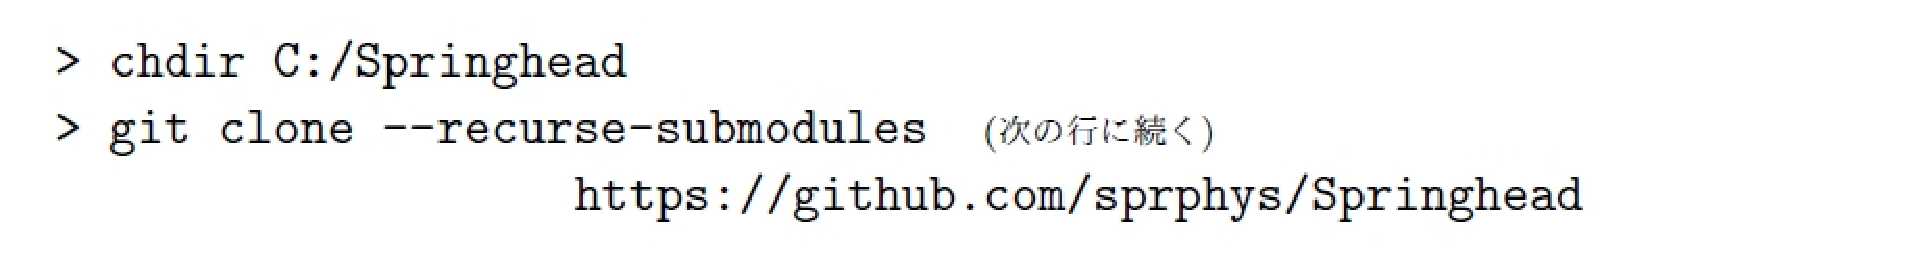
\includegraphics[width=\textwidth]{fig/command-2-1-a.eps}
	    \end{center}
	    \label{fig:DownloadTree}
	\end{figure}
\else
\begin{narrow}[15pt]
	\CmndBox{%
		> chdir C:/Springhead\\
		> git clone --recurse-submodules\Cont\\
		\Hskip{100pt}https://github.com/sprphys/Springhead
	}
\end{narrow}
\fi
\medskip
サブモジュールを選択する場合は、
\ifLwarp
	\begin{figure}[h]
	    \begin{center}
	    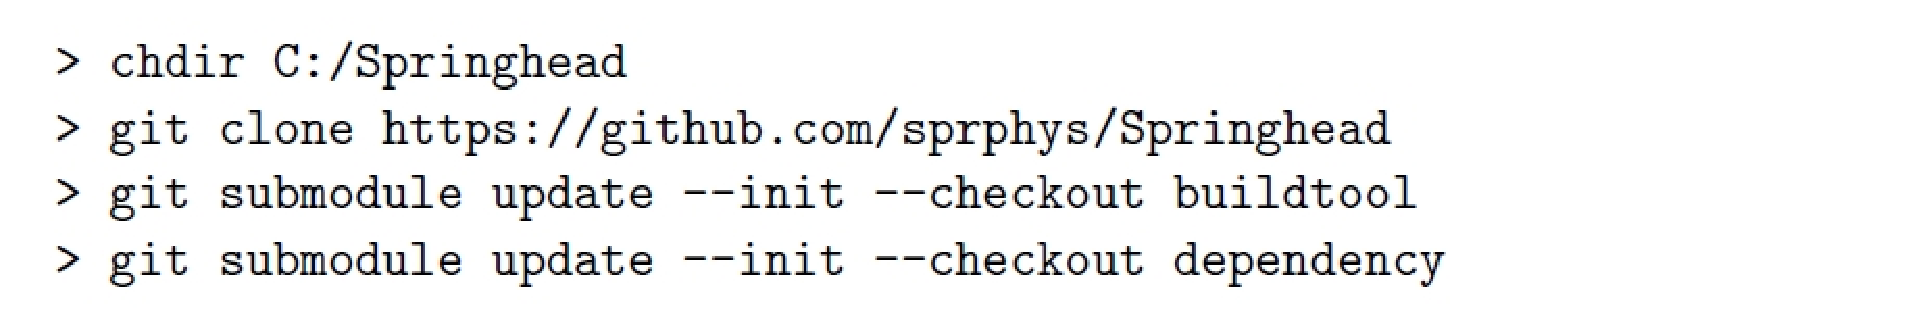
\includegraphics[width=\textwidth]{fig/command-2-1-b.eps}
	    \end{center}
	    \label{fig:DownloadTree}
	\end{figure}
\else
\begin{narrow}[15pt]
	\CmndBox{%
		> chdir C:/Springhead\\
		> git clone https://github.com/sprphys/Springhead\\
		> git submodule update --init --checkout buildtool\\
		> git submodule update --init --checkout dependency
	}
\end{narrow}
\fi
\medskip
GUIの場合は、
\begin{narrow}[15pt]
	\begin{figure}[h]
	\begin{center}
	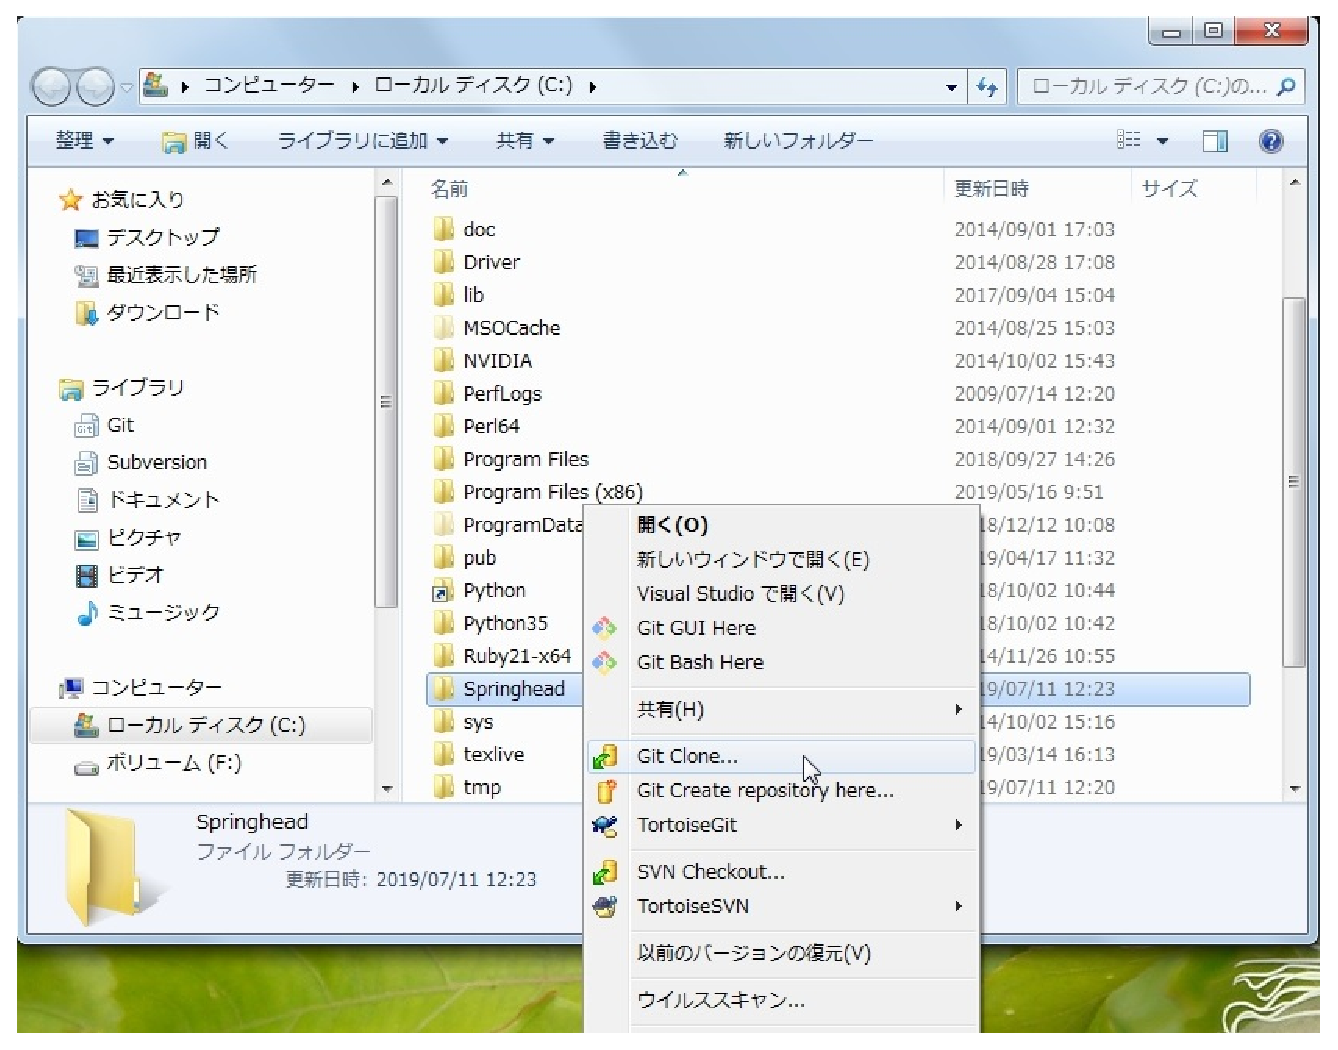
\includegraphics[width=0.5\textwidth]{fig/SpringheadClone1.eps}
	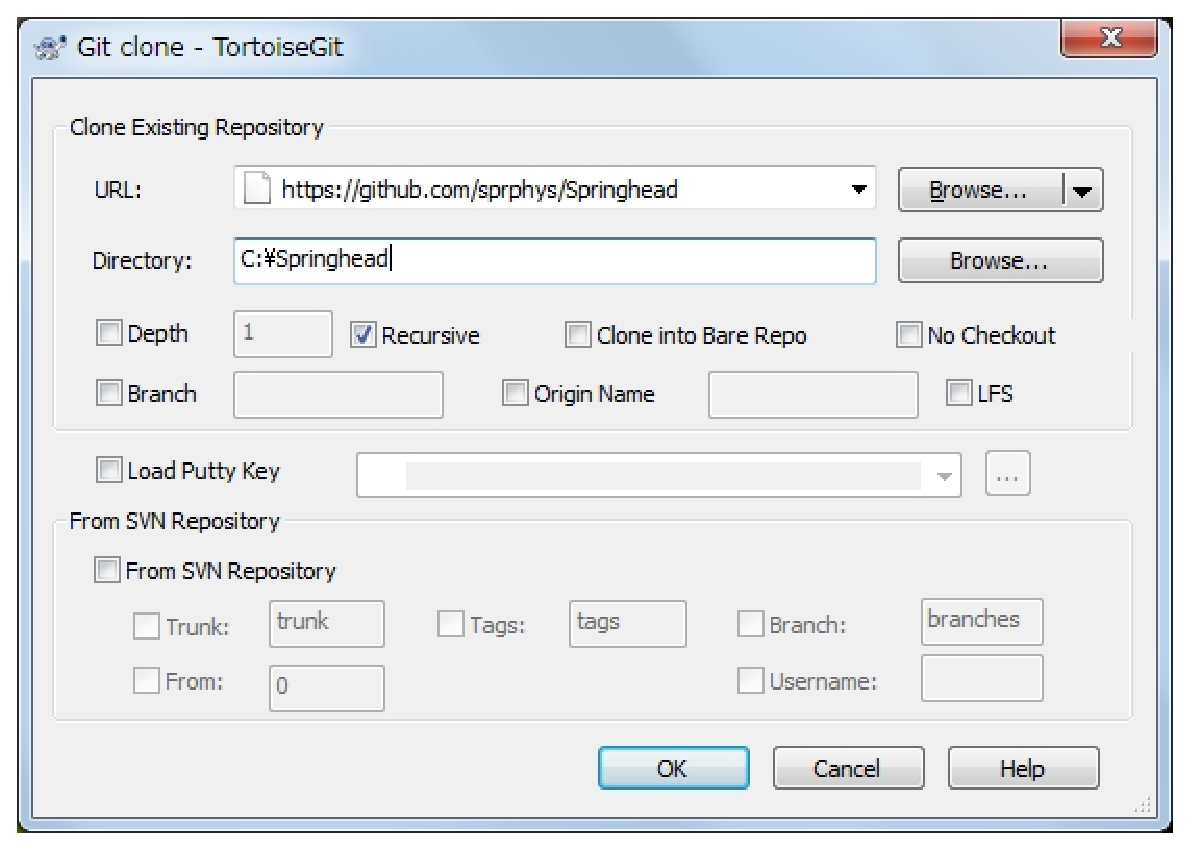
\includegraphics[width=0.4\textwidth]{fig/SpringheadClone2.eps}
	\end{center}
	\caption{Springheadダウンロード}
	\label{fig:SpringheadClone}
	\end{figure}
\end{narrow}

% end: 2.1.Download.tex

% 2.2.PrepareLibrary.tex
%	Last update: 2019/07/24 F.Kanehori
%newpage
\subsection{K11cOJIYzUE65BBo}
\label{subsec:PrepareLibrary}

\noindent
\KLUDGE ダウンロードが済んだら\SprTop{/core/src}\KLUDGE に移動してください。

\noindent
\KLUDGE まず、配布されたファイル\CMakeLists{.Lib.dist}\KLUDGE を
\CMakeLists{}\KLUDGE という名前でコピーします
(\KLUDGE 誤コミットを防止するためにもリネームではなくコピーしてください)。

\medskip
\ifLwarp
	\begin{figure}[h]
	    \begin{center}
	    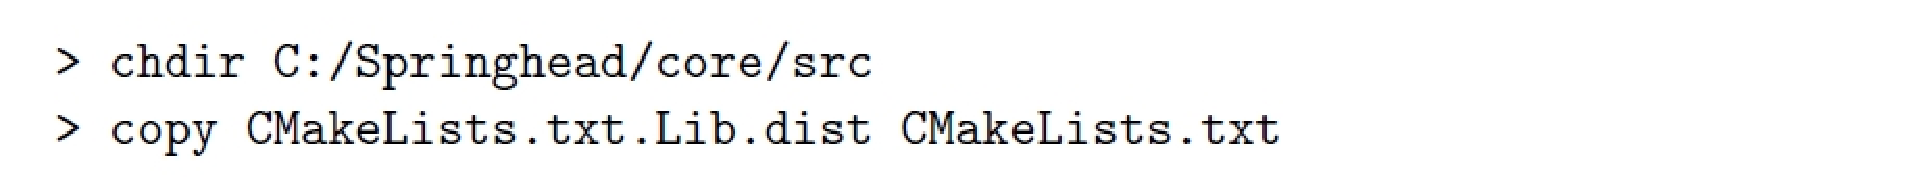
\includegraphics[width=\textwidth]{fig/command-2-2-a.eps}
	    \end{center}
	    \label{fig:DownloadTree}
	\end{figure}
\else
\begin{narrow}[15pt]
	\CmndBox{%
		\textgreater  chdir C:/Springhead/core/src\\
		\textgreater  copy CMakeLists.txt.Lib.dist CMakeLists.txt
	}
\end{narrow}
\fi

\medskip
\noindent
\KLUDGE 自前でインストールしているパッケージ
(\tt{boost}, \tt{glew}, \tt{freeglut}, \tt{glui})\KLUDGE を使用する場合
\KLUDGE およびライブラリファイルとヘッダファイルのインストール先を指定する場合には、
\KLUDGE さらに、
\KLUDGE 配布されたファイル\CMakeConf{.dist}\KLUDGE を\CMakeConf{}\KLUDGE という名前でコピーして
\KLUDGE 必要な編集をします。
\KLUDGE 編集の方法については\CMakeConf{}\KLUDGE に記述されています
(``\tt{=ESCAPEx23=set(variable \it{value})}''\KLUDGE から``\tt{=ESCAPEx23=}''\KLUDGE を削除し、
``\it{value}''\KLUDGE を適切に設定し直す)\KLUDGE 。

\def\cite=ESCAPEx23=1{\hspace{10pt}\footnotesize{=ESCAPEx23=1}}
\def\somewhere{"C:/\it{somewhere}/\it{appropreate}"}
\medskip
\ifLwarp
	\begin{figure}[h]
	    \begin{center}
	    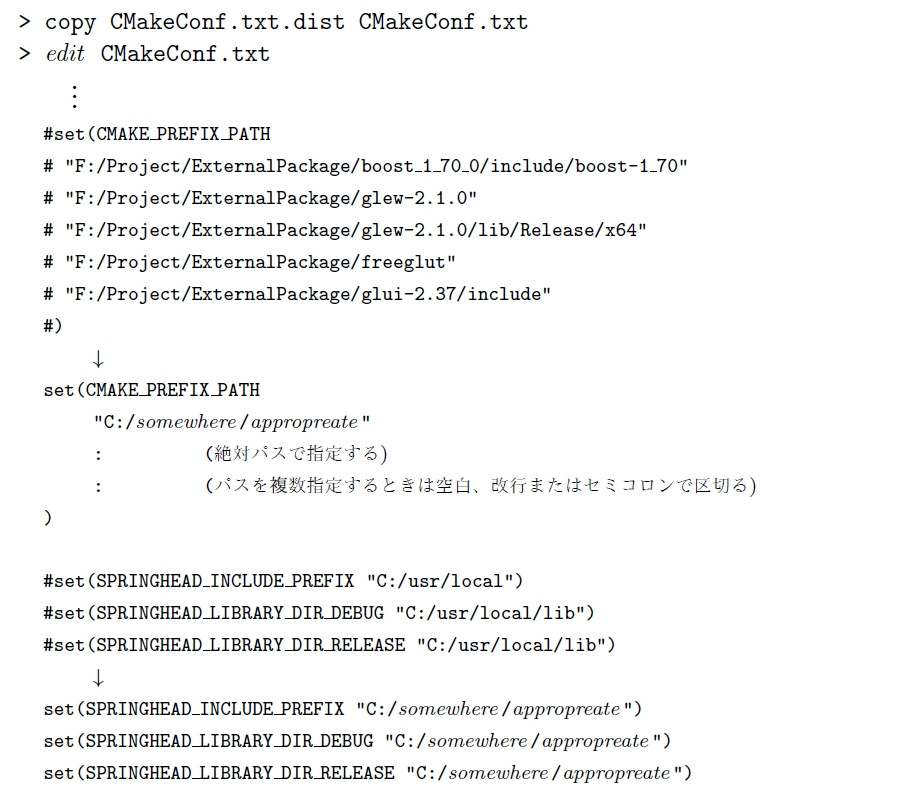
\includegraphics[width=\textwidth]{fig/command-2-2-b.eps}
	    \end{center}
	    \label{fig:DownloadTree}
	\end{figure}
\else
\begin{narrow}[15pt]
	\CmndBox{%
		\textgreater  copy CMakeConf.txt.dist CMakeConf.txt\\
		\textgreater  \it{edit} CMakeConf.txt\\
		\hspace{20pt}$\vdots$\\
	\cite{=ESCAPEx23=set(CMAKE\_PREFIX\_PATH}\\
	\cite{=ESCAPEx23= "F:/Project/ExternalPackage/boost\_1\_70\_0/include/boost-1\_70"}\\
	\cite{=ESCAPEx23= "F:/Project/ExternalPackage/glew-2.1.0"}\\
	\cite{=ESCAPEx23= "F:/Project/ExternalPackage/glew-2.1.0/lib/Release/x64"}\\
	\cite{=ESCAPEx23= "F:/Project/ExternalPackage/freeglut"}\\
	\cite{=ESCAPEx23= "F:/Project/ExternalPackage/glui-2.37/include"}\\
	\cite{=ESCAPEx23=)}\\
	\cite{\hspace{20pt}$\downarrow$}\\
	\cite{set(CMAKE\_PREFIX\_PATH}\\
	\cite{\hbox to 20pt{}\somewhere}\\
	\cite{\hspace{20pt}:\hspace{40pt}{(\rm{\KLUDGE 絶対パスで指定する)}}}\\
	\cite{\hspace{20pt}:\hspace{40pt}%
		{(\rm{\KLUDGE パスを複数指定するときは空白、改行またはセミコロンで区切る)}}}\\
	\cite{)}\\
	\cite{}\\
	\cite{=ESCAPEx23=set(SPRINGHEAD\_INCLUDE\_PREFIX       "C:/usr/local")}\\
	\cite{=ESCAPEx23=set(SPRINGHEAD\_LIBRARY\_DIR\_DEBUG   "C:/usr/local/lib")}\\
	\cite{=ESCAPEx23=set(SPRINGHEAD\_LIBRARY\_DIR\_RELEASE "C:/usr/local/lib")}\\
	\cite{\hspace{20pt}$\downarrow$}\\
	\cite{set(SPRINGHEAD\_INCLUDE\_PREFIX       \somewhere)}\\
	\cite{set(SPRINGHEAD\_LIBRARY\_DIR\_DEBUG   \somewhere)}\\
	\cite{set(SPRINGHEAD\_LIBRARY\_DIR\_RELEASE \somewhere)}
	}
\end{narrow}
\fi

\medskip
\noindent
\KLUDGE 以上で準備作業は終了です。

% end: 2.2.PrepareLibrary.tex

% 2.3.CmakeLibrary.tex
%	Last update: 2019/07/24 F.Kanehori
%newpage
\subsection{cmakeの実行}
\label{subsec:CmakeLibrary}

\noindent
以下では、\cmake の生成物(ビルドの生成物ではありません)を格納する
作業場所(ディレクトリ)を``\build''として話を進めます(作業場所は任意で構いません)。

\medskip
\noindent
\cmake にはConfigureとGenerateの2段階があります。

\medskip
\noindent
コマンドプロンプトの場合は、1回のコマンドで両方を実行できます。
\Vskip{-.5\baselineskip}
\ifLwarp
	\begin{figure}[h]
	    \begin{center}
	    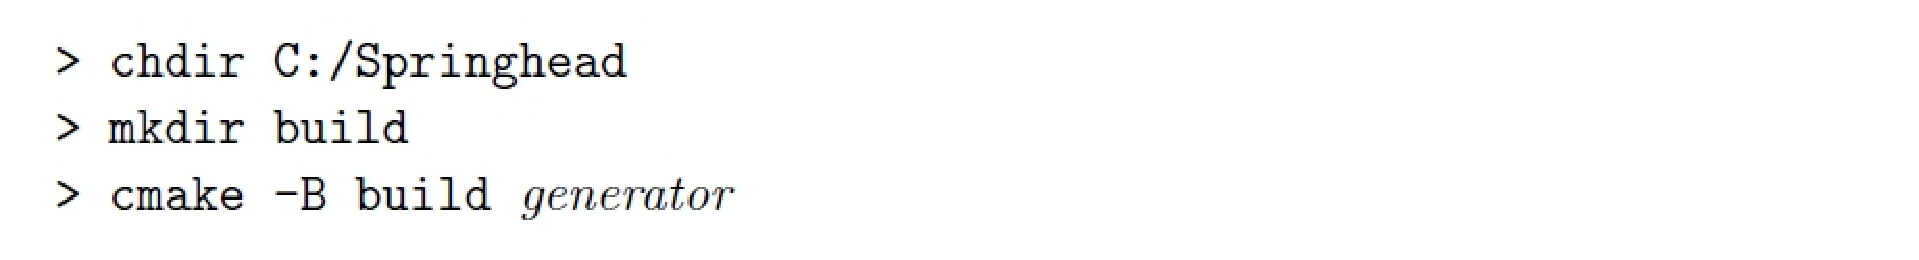
\includegraphics[width=\textwidth]{fig/command-2-3.eps}
	    \end{center}
	    \label{fig:DownloadTree}
	\end{figure}
\else
\begin{narrow}[15pt]
	\CmndBox{%
		> chdir C:/Springhead\\
		> mkdir build\\
		> cmake -B build \it{generator}
	}
	\it{generatorの}詳細(\KQuote{\tt{-G "Visual Studio 15 2017" -A x64}}など)は、
	コマンドプロンプトで\tt{cmake --help}とすると確認できます。
\end{narrow}
\fi

\medskip
\noindent
GUIの場合は、
\begin{narrow}[15pt]
	まずConfigureボタン(図\ref{fig:CmakeConfigure} 左図の下)を押します。
	\begin{figure}[h]
	\begin{center}
	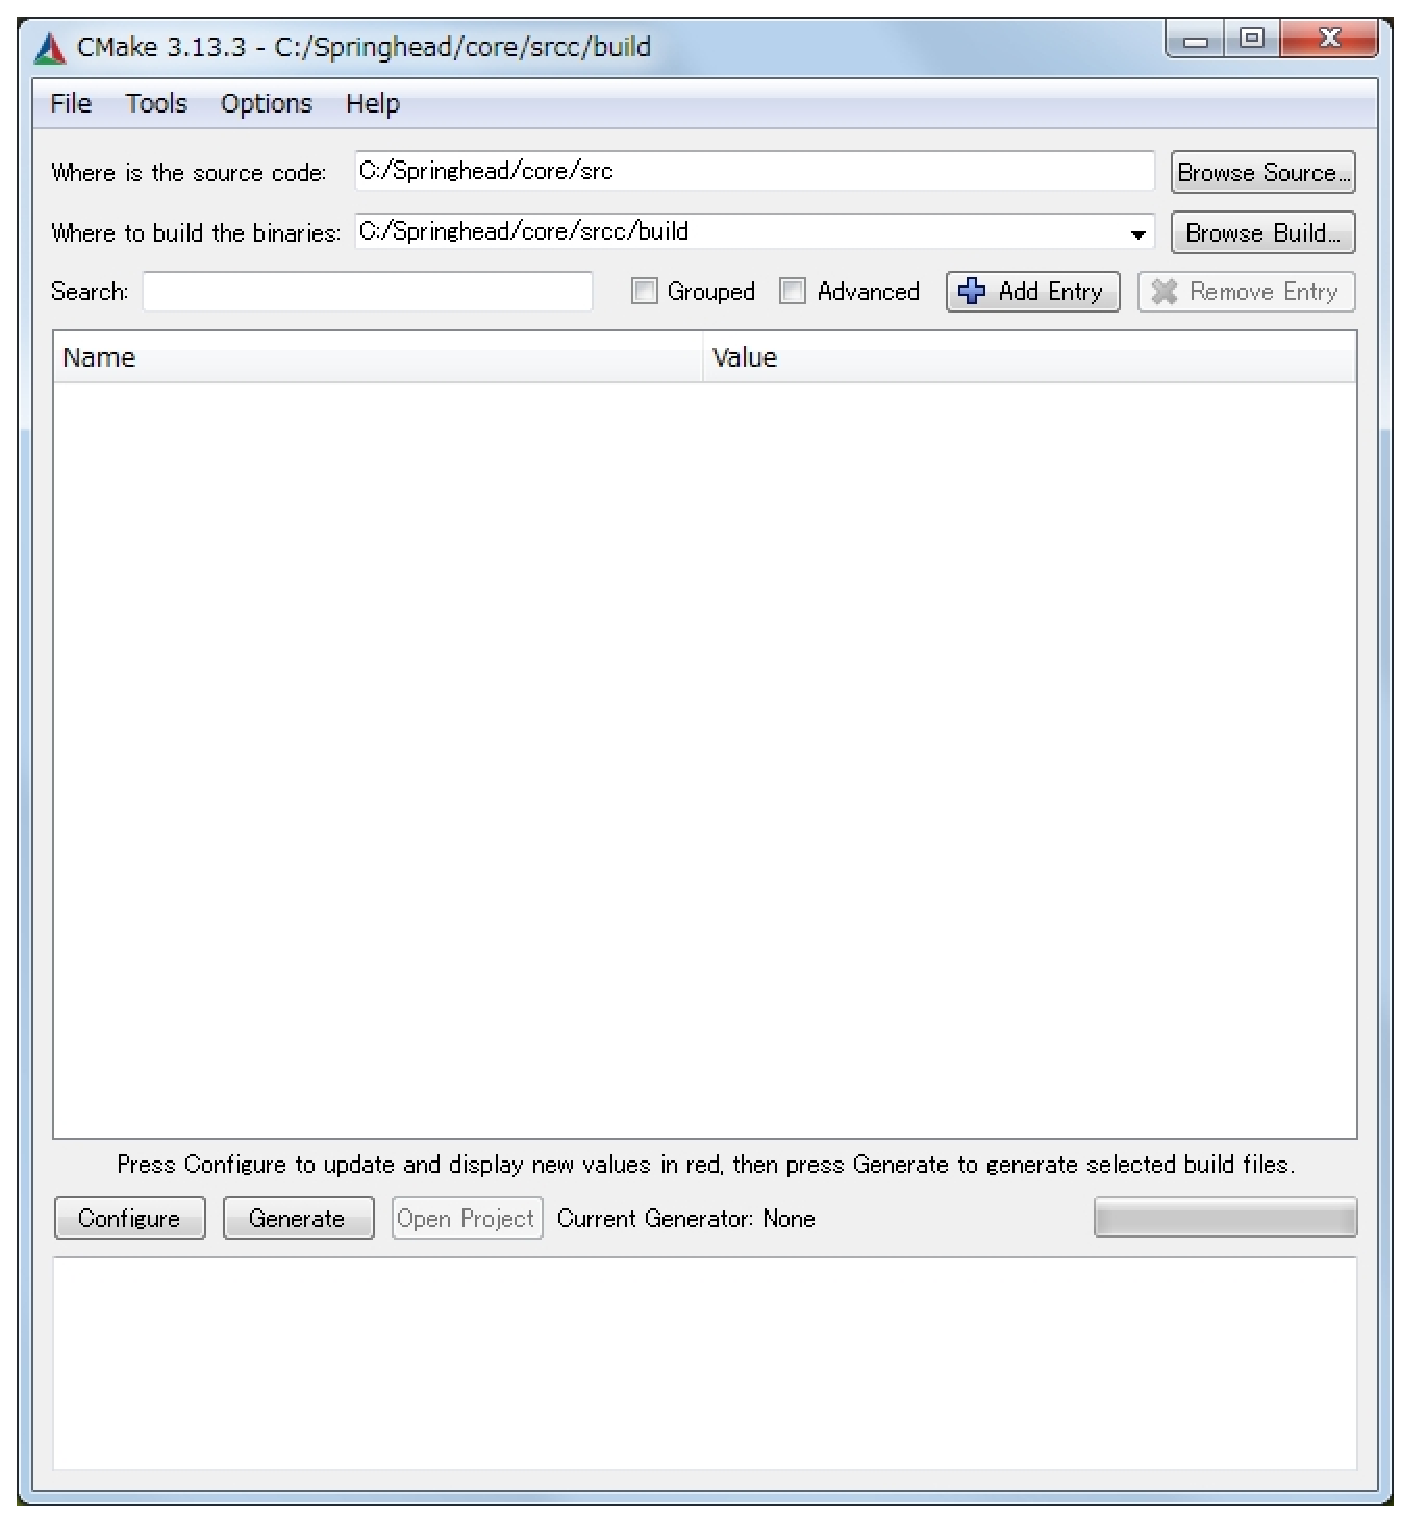
\includegraphics[width=0.35\textwidth]{fig/CmakeConfigure1.eps}
	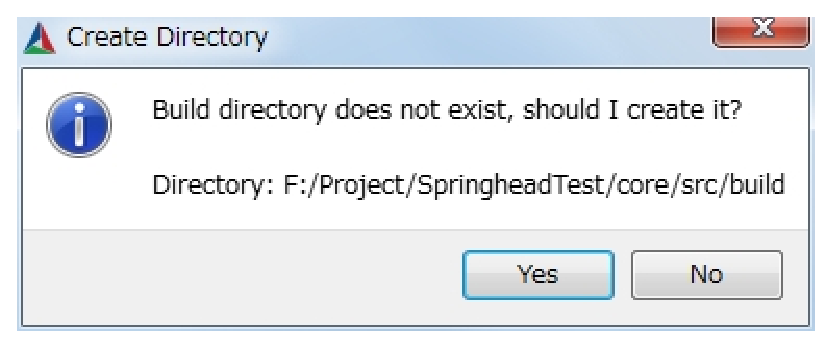
\includegraphics[width=0.2\textwidth]{fig/CmakeConfigure2.eps}
	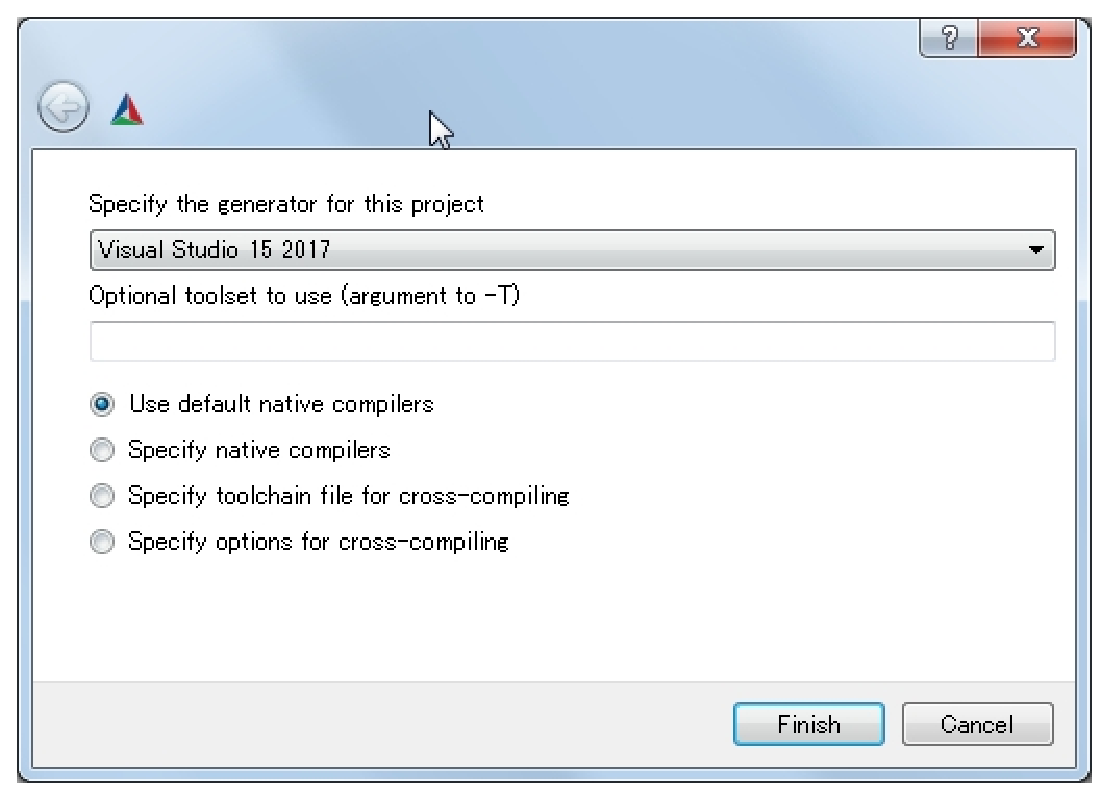
\includegraphics[width=0.3\textwidth]{fig/CmakeConfigure3.eps}
	\end{center}
	\caption{\cmake\ configure}
	\label{fig:CmakeConfigure}
	\end{figure}

	\Vskip{-.5\baselineskip}
	\build ディレクトリがなければ作成するかどうか聞かれ(同中央図)、
	次にgenerator指定画面となります(同右図)。
	cmake version 3.15.0では、
	generatorとして図\ref{fig:CmakeGenerator}のものが指定できます。

	\begin{figure}[h]
	\begin{center}
	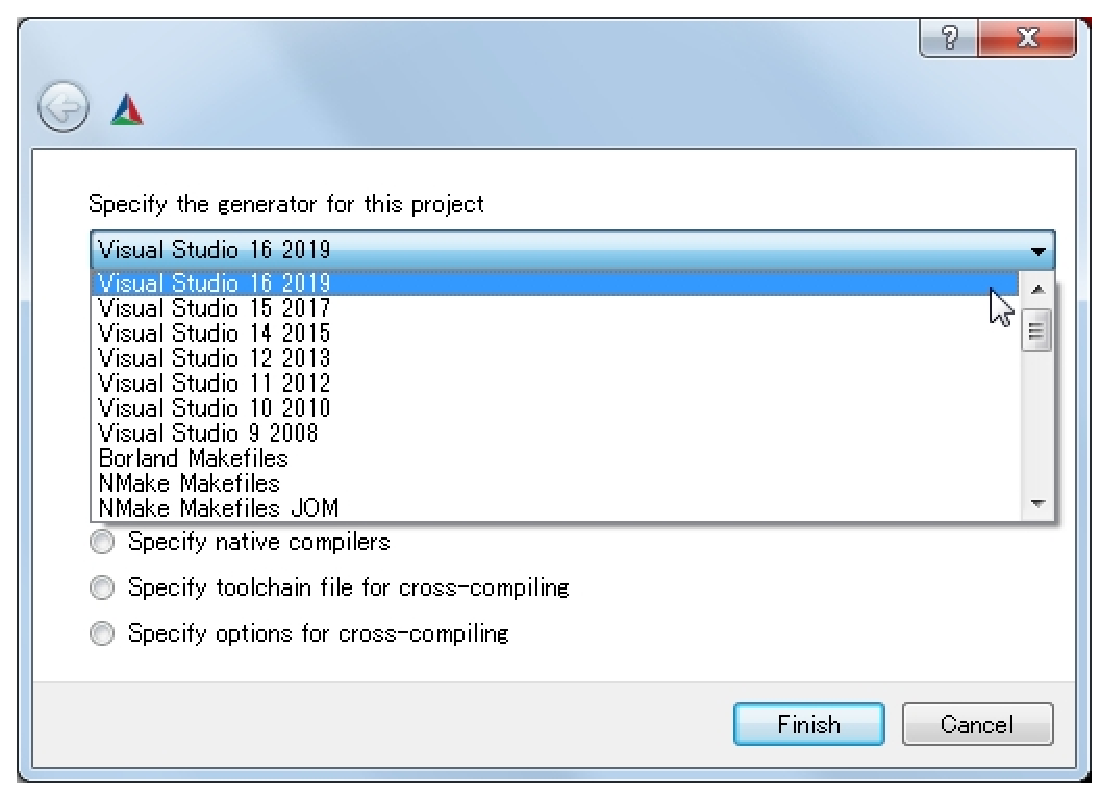
\includegraphics[width=0.3\textwidth]{fig/CmakeConfigure4.eps}
	\end{center}
	\caption{\cmake\ generator}
	\label{fig:CmakeGenerator}
	\end{figure}

	最後に図\ref{fig:CmakeConfigure} 左図の下のGenerateボタンを押します。
\end{narrow}

\medskip
\noindent
以上で、\build 以下にsolution/project fileなどが生成されたはずです。

\bigskip

% end: 2.3.CmakeLibrary.tex

% 2.4.BuildLibrary.tex
%	Last update: 2019/07/11 F.Kanehori
%newpage
\subsection{ライブラリのビルド}
\label{subsec:BuildLibrary}

\noindent
Springhead Libraryのビルドは、従来と変わりがありません。\\
\build へ移動し、\Path{Spsringhead.sln}を指定してVisual Studioを実行してください。

\medskip
``\ref{subsec:PrepareLibrary} 準備''でライブラリファイルのインストール先を
指定していないときは、\\
\SprTop{/generated/lib/win64}または\SprTop{/generated/lib/win32}\\
にライブラリファイルが生成されます。

% end: 2.4.BuildLibrary.tex

%
% 3.0.ForDevelopper.tex
%	Last update: 2019/07/17 F.Kanehori
\newpage
\section{Springheadを開発する方へ}
\label{sec:ForDevelopper}

\noindent
この章では、Springheadの開発を行なう方のために、
\cmake を使用したアプリケーションプログラムの作成方法について説明します。

\medskip
アプリケーションプログラムについての作業をする前に、
あらかじめSpringehadライブラリをダウンロードして\cmake を実行しておいてください
(\KQuote{\ref{sec:ForNonDevelopper} Springheadをライブラリとして利用する方へ}参照)。

% end: 3.0.ForDevelopper.tex

% 3.1.PrepareApplication.tex
%	Last update: 2019/10/03 F.Kanehori
%\newpage
\subsection{sByVELhUuWQYiYYM}
\label{subsec:PrepareApplication}

\noindent
\KLUDGE アプリケーションと並行してSpringhead\KLUDGE ライブラリを開発する場合には、
\KQuoteS\ref{subsec:Problems} CMake\KLUDGE を使用した場合の問題点\KQuoteE
\KLUDGE で示した問題に対処する必要があるため、
\KLUDGE ここで述べる方法に従って作業を進めてください
(\KQuote{\ref{subsec:Solution} \KLUDGE 対処法}\KLUDGE で示した方策が組み込まれます)\KLUDGE 。

\medskip
\KLUDGE 以下、Springhead\KLUDGE ライブラリをダウンロードしたディレクトリを\SprTop{} \KLUDGE 、
\KLUDGE アプリケーションプログラムを作成するディレクトリを\AppTop{}\KLUDGE として説明を進めます。

\bigskip
\noindent
\AppTop{}\KLUDGE に移動してください。

\bigskip
\noindent
\KLUDGE 配布されたファイル\CMakeTopdir{.dist}\KLUDGE を\CMakeTopdir{}\KLUDGE という名前で、
\CMakeLists{.Dev.dist}\KLUDGE を\CMakeLists{}\KLUDGE という名前でコピーします
(\KLUDGE 誤ってコミットするのを防ぐためにも、リネームではなくコピーしてください)。

\medskip
\ifLwarp
	\begin{figure}[h]
	    \begin{center}
	    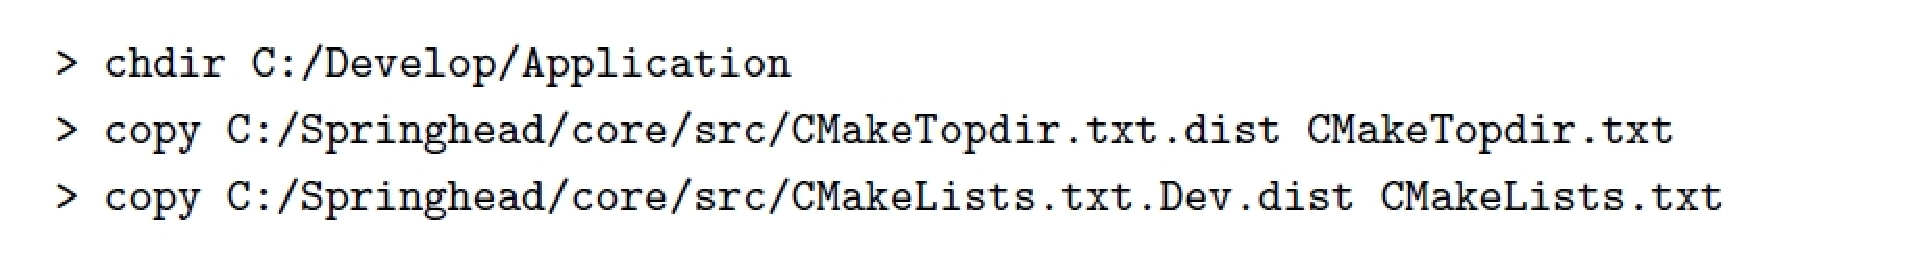
\includegraphics[width=\textwidth]{fig/command-3-1-a.eps}
	    \end{center}
	    \label{fig:DownloadTree}
	\end{figure}
\else
\begin{narrow}[15pt]
	\CmndBox{%
	{\small{\textgreater  chdir C:/Develop/Application}}\\
	{\small{\textgreater  copy C:/Springhead/core/src/CMakeTopdir.txt.dist CMakeTopdir.txt}}\\
	{\small{\textgreater  copy C:/Springhead/core/src/CMakeLists.txt.Dev.dist CMakeLists.txt}}
	}
\end{narrow}
\fi

\bigskip
\noindent
\bf{\CMakeTopdir{}}\KLUDGE の編集
\begin{narrow}[20pt]
	\SprLib \KLUDGE をダウンロードしたディレクトリを\CMakeTopdir{}\KLUDGE には\SprLib \KLUDGE に設定します。
	\KLUDGE これは、CMake\KLUDGE にSpringhead\KLUDGE のソースツリーの場所を教えるために必要な設定です。

\ifLwarp
	\begin{figure}[h]
	    \begin{center}
	    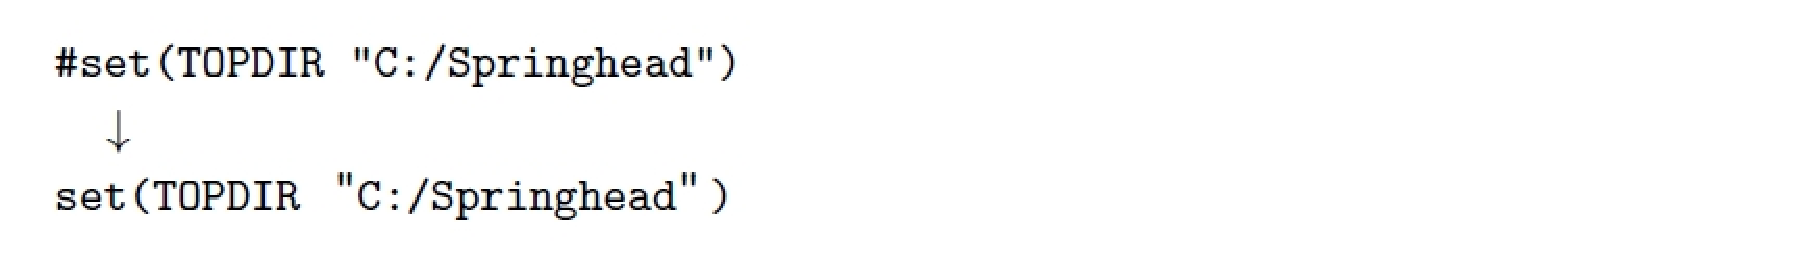
\includegraphics[width=\textwidth]{fig/command-3-1-b.eps}
	    \end{center}
	    \label{fig:DownloadTree}
	\end{figure}
\else
	\begin{narrow}[15pt]
		\CmndBox{%
			{\small{=ESCAPEx23=set(TOPDIR "C:/Springhead")}}\\
			\hspace{10pt}{\small{$\downarrow$}}\\
			{\small{set(TOPDIR \SprTop{})}}
		}
	\end{narrow}
\fi
\end{narrow}
\medskip
\noindent
\bf{\CMakeLists{}}\KLUDGE の編集
\begin{narrow}[20pt]
	\begin{enumerate}
	    \item
		\KLUDGE プロジェクト名を設定します(11\KLUDGE 行目)\KLUDGE 。

\ifLwarp
		\begin{figure}[h]
			\begin{center}
			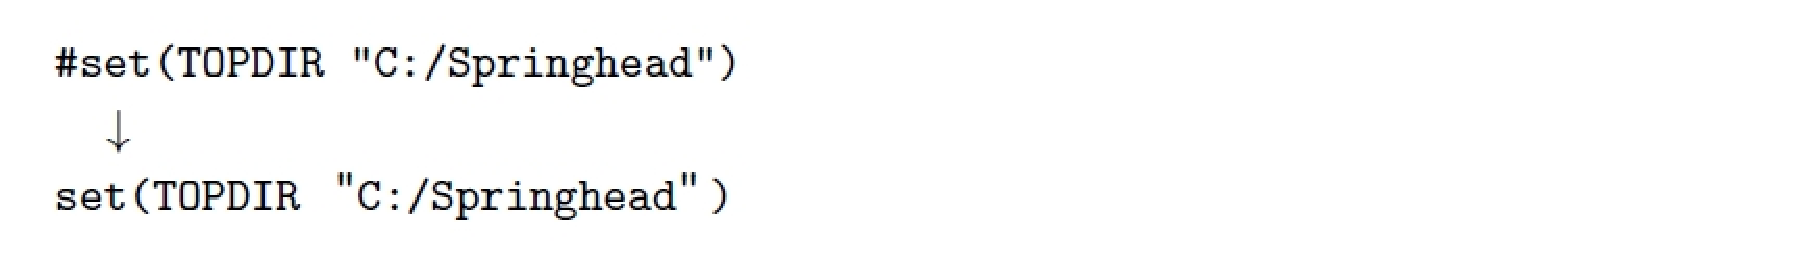
\includegraphics[width=\textwidth]{fig/command-3-1-b.eps}
				\end{center}
			\label{fig:DownloadTree}
		\end{figure}
\else
		\begin{narrow}[s][5pt]
			\CmndBox{%
				{\small{set(ProjectName "Project")}}\\
				\hspace{10pt}{\small{$\downarrow$}}\\
				{\small{set(ProjectName "\textless \it{MyApplication}\textgreater ")}}
			}
		\end{narrow}
		\Vskip{.5\baselineskip}
\fi

	    \item
		Customization section (19\KLUDGE 行目以降)\KLUDGE を必要に応じて変更します。\\
		\KLUDGE 各変数の意味は次のとおりです。

		\medskip
		\def\SetRelPath{\tt{RELATIVE \$\{CMAKE\_SOURCE\_DIR\}}}
		\def\CMakeSrcDir{\tt{\$\{CMAKE\_SOURCE\_DIR\}}}
		\def\Explanation=ESCAPEx23=1{\begin{minipage}[t]{222pt}{=ESCAPEx23=1}\end{minipage}}

		\begin{narrow}[4pt]
		\begin{tabular}{|l|l|}\hline
		    \tt{OOS\_BLD\_DIR} &
			%\begin{minipage}[t]{220pt}
			%CMake\KLUDGE の作業領域(\KLUDGE ディレクトリ)\KLUDGE の名前(\KLUDGE 本ドキュメントで
			%\build \KLUDGE としているもの)\KLUDGE 。
			%\end{minipage}
			%\\\hline
			CMake\KLUDGE の作業領域(\KLUDGE ディレクトリ)\KLUDGE の名前(\KLUDGE 本ドキュ\\
			& \KLUDGE メントで\build \KLUDGE としているもの)\KLUDGE 。\\\hline
		    \multicolumn{2}{|l|}{%
			\tt{CMAKE\_CONFIGURATION\_TYPES}} \\
			& \KLUDGE ビルド構成。\\\hline
		    \tt{SRCS} &
			\KLUDGE ビルドの対象とするファイル。
			\KLUDGE 設定は\tt{set(SRCS \KLUDGE …)} \\
			& \KLUDGE または\tt{file(GLOB SRCS \KLUDGE …)}\KLUDGE とします。\\
			& \KLUDGE 後者ではワイルドカードが使えます。\\
			& \tt{SRCS}\KLUDGE の直後に``\tt{RELATIVE \textless \it{base-dir}\textgreater }''\KLUDGE を付加すると \\
			& \KLUDGE 相対パス指定となります。デフォルトは \\
			& \ \ {\footnotesize{\tt{file(GLOB \SetRelPath\ *.cpp *.h)}}} \\
			& \KLUDGE です。\\\hline
		    \tt{EXCLUDE\_SRCS} &
			\KLUDGE ビルドの対象から外すファイル。\\
			& \KLUDGE 上の\tt{SRCS}\KLUDGE で\tt{RELATIVE}\KLUDGE としていないときは絶対パス \\
			& \KLUDGE で指定します。\\
			& \tt{SRCS}\KLUDGE でワイルドカードを使用した場合に有用です。\\\hline
		    \tt{SPR\_PROJS} &
			\KLUDGE アプリケーションに組み込むSpringhead\KLUDGE ライブラリ\\
			& \KLUDGE のプロジェクト名。\\
			& \KLUDGE 不要なプロジェクト名を削除します。
			\KLUDGE この中にRun-\\
			& Swig\KLUDGE を含めてはいけません。\\\hline
		    \tt{ADDITIONAL\_INCDIR} &
			\KLUDGE 追加のインクルードパス指定。\\
			& \KLUDGE 現在のディレクトリは \CMakeSrcDir \KLUDGE で参照 \\
			& \KLUDGE できます。\\\hline
		    \tt{ADDITIONAL\_LIBDIR} &
			\KLUDGE 追加のライブラリパス指定。\\\hline
		    \tt{ADDITIONAL\_LIBS} &
			\KLUDGE 追加のライブラリファイル名。\\\hline
		    \tt{EXCLUDE\_LIBS} &
			link\KLUDGE の対象から外すライブラリファイル名。\\
			& \KLUDGE デフォルトで組み込まれてしまうライブラリファイル\\
			& \KLUDGE を排除するために指定します。\\\hline
\ifLwarp\else
		\end{tabular}
		\begin{tabular}{|l|l|}\hline
\fi
		    \multicolumn{2}{|l|}{%
			\tt{DEBUGGER\_WORKING\_DIRECTORY}} \\
			\phantom{\tt{ADDITIONAL\_INCDIR}}
			& Visual Studio Debugger\KLUDGE の作業ディレクトリ名。\\
			& \KLUDGE デバッガはこのディレクトリで起動されたように振る \\
			& \KLUDGE 舞います。\\\hline
		    \multicolumn{2}{|l|}{%
			\tt{DEBUGGER\_COMMAND\_ARGUMENTS}} \\
			& Visual Studio Debugger\KLUDGE に渡すコマンド引数 \\\hline
		\end{tabular}
		\end{narrow}
	\end{enumerate}
\end{narrow}

\bigskip
\noindent
\KLUDGE 自前でインストールしているパッケージ
(\tt{boost}, \tt{glew}, \tt{freeglut}, \tt{glui})\KLUDGE を使用する場合には、
\KLUDGE さらに、
\KLUDGE 配布されたファイル\CMakeConf{.dist}\KLUDGE を\CMakeConf{}\KLUDGE という名前でコピーして
\KLUDGE 必要な編集をします。
\KQuote{\ref{subsec:PrepareLibrary} \KLUDGE 準備}\KLUDGE を参照してください。

\medskip
\noindent
\KLUDGE ビルドの条件(compile/link\KLUDGE のパラメータ)\KLUDGE を変更したいときは、
\KLUDGE 配布されたファイル\CMakeOpts{.dist}\KLUDGE を\CMakeOpts{}\KLUDGE という名前でコピーして
\KLUDGE 適宜変更してください。

\medskip
\noindent
\KLUDGE 以上で準備作業は終了です。

% end: 3.1.PrepareApplication.tex

% 3.2.CmakeApplication.tex
%	Last update: 2019/10/07 F.Kanehori
%newpage
\subsection{cmakeの実行}
\label{subsec:CmakeApplication}

\noindent
\cmake の実行手順については、
\KQuote{\ref{subsec:CmakeLibrary} cmakeの実行}と同じですから、
そちらを参照してください。
ここでは、\cmake を実行することで
\KQuote{\ref{subsec:Solution} 対処法}で示した対策がどのように実施されるかについて述べます。

\bigskip
\noindent
\bf{ビルドの最適性}
\begin{narrow}[20pt]
	組み込まれているSpringheadライブラリの各プロジェクト
	(ここでは\tt{Base}を例にします)に対して\\
	\hspace{20pt}\SprTop{/core/src/Base/\it{\textless x64\textgreater}/%
		\it{\textless 15.0\textgreater}/Base.dir}\Note{(*1)}\\
	というディレクトリを作成し、
	\AppTop{/\build /Base/Base.dir}から上記ディレクトリ\Note{(*1)}へ
	linkを張る作業を\cmake\ configure時に(自動的に)行ないます。
\end{narrow}	
\begin{narrow}[20pt]
	\thinrule{\linewidth}\\
	{\bf{これに関して皆さんが行なうべきことはありませんが、
	次のことに注意してください。}}

	\medskip
	\begin{enumerate}
	  \item	\cmake をした後でSpringheadソースツリー上ので上記ディレクトリ
		\Note{(*1)}を削除すると、以降のビルドで\\
		\hspace{15pt}\KQuote{\tt{\small{%
		エラー MSB3191 ディレクトリ\Path{Base.dir/Debug/}を作成できません。}}}

		というエラーが発生します。

	  \item	\SprLib 側で\cmake\ (configure)を実行していないと
		オブジェクトの共通格納領域が作成されていないため、
		前項と同じエラーが発生します。

	  \item	アプリケーション側で\AppTop{/\build /Base/Base.dir}を削除すると、
		ビルド時にVisual Studioが\build 下に\Path{Base.dir}を
		自動的に作成するためにビルドの最適性が崩れてしまいます
		(無駄なビルドが発生するだけで、ビルド自体は正常に行なえます)。
		\begin{narrow}[s][15pt]
		Windowsでは実行権限の都合上linkをjunctionで実現していますが、
		explorerでもcommand prompt上でも\Path{Base.dir}がjunctionか
		通常のディレクトリかの区別がつきません。
		そのためこのような事態の発見が困難になる可能性があります。
		\end{narrow}
	\end{enumerate}
	\medskip
	{\bf{これらの状態を解消するためには、アプリケーション側
	(もしくはSpringheadライブラリ側)で再度\cmake を実行する必要があります。}}

	\thinrule{\linewidth}
\end{narrow}

\bigskip
\noindent
\bf{プロジェクトファイルの整合性}
\begin{narrow}[20pt]
	\KQuote{\ref{subsec:Solution} 対処法}でも述べたように、
	プロジェクトファイル(ソリューションファイルの含む。以下同様)は
	Springheadライブラリのビルドツリーにあるものを最新の状態に保つことを前提として、
	アプリケーション側のプロジェクトファイルは
	これらSpringhead側にあるものへのlinkとなるようにします。
	このためにアプリケーションプログラムのソリューションに
	\tt{sync}というターゲットを追加して、次の処理を実行させます。
	\begin{enumerate}
	  \item	もしもアプリケーション側のプロジェクトファイルの内容と
		Springhead側のプロジェクトファイルの内容とが異なっていたならば、
		アプリケーション側のプロジェクトファイルを
		Springhead側にコピーする。
		\begin{narrow}[s][15pt]
		これは、アプリケーション側でソースファイル構成を変更
		(ファイルの追加・削除)を行ない、
		Visual Studio上でプロジェクトファイルを保存したとき、
		またはアプリケーション側で再度\cmake を実行したときです。
		\end{narrow}

	  \item	アプリケーション側のプロジェクトファイルをSpringhead側の
		プロジェクトファイルへのlinkとする。
	\end{enumerate}
	ターゲット\tt{sync}はアプリケーションのビルドにおいて
	必ず最初に実行されるように依存関係が設定されます。
\end{narrow}	
\begin{narrow}[20pt]
	\thinrule{\linewidth}\\
	{\bf{次のことに注意してください。}}

	\medskip
	\begin{enumerate}
	  \item	Springhead側または他のアプリケーションが実施した変更は、
		アプリケーションをビルドするだけで自動的に反映されます。

	  \item	自アプリケーションで実施したソース構成の変更は、
		ビルドを実施した時点でSpringhead側に反映されます。
		つまり、プロジェクトファイルの整合性を保つためには、
		ソース構成の変更後に少なくとも1回はビルドを実行する必要がある
		ということです(\tt{sync}の実行だけでもよい)。
		\begin{narrow}[s][15pt]
		ソース構成を変更したらビルドするでしょうから、
		このことが問題になることはほとんどないと思われます。

		もしSpringhead側でプロジェクトファイルが削除されたならば、
		ビルドエラー(\tt{sync}でlink先のファイルが見つからない)
		となります。
		
		{\bf{この場合にはSpringhead側で再度\cmake を実行する必要があります
		(アプリケーション側では駄目)。}}
		\end{narrow}

	  \item	\tt{sync}ターゲットが実行されるとプロジェクトファイルが更新される
		ことがあるため、\KQuoteS プロジェクトが環境外で変更された\KQuoteE 旨の
		メッセージが出ることがあります。
		「すべて再読み込み」としてください。
	\end{enumerate}

	\thinrule{\linewidth}
\end{narrow}	

% end: 3.2.CmakeApplication.tex

% 3.3.BuildApplication.tex
%	Last update: 2019/10/07 F.Kanehori
%newpage
\subsection{R8w47HeMnww1Wqw5}
\label{subsec:BuildApplication}

\noindent
\KLUDGE アプリケーションのビルドは従来と変わりがありませんが、
\KLUDGE ソリューションに新しいターゲット
\tt{ALL\_BUILD}, \tt{sync}\KLUDGE が追加されています。
\KLUDGE ここでは、これらについて説明します。

\medskip
\noindent
\tt{ALL\_BUILD}
\begin{narrow}[20pt]
	\KLUDGE これは\cmake \KLUDGE が自動的に作成するターゲットでmake all\KLUDGE に相当するものと
	\KLUDGE されています。ただしVisual Studio\KLUDGE 上ではALL\_BUILD\KLUDGE の依存関係の設定が不正確で、
	\KLUDGE このターゲットをビルドしても正しい結果は得られないようです。
	{\bf{\KLUDGE このターゲットは無視してください}}
\end{narrow}

%\noindent
%\tt{RunSwig\_Clean} \\
%\tt{EmbPython\_RunSwig\_Clean}
%\begin{narrow}[20pt]
%	\KLUDGE 従来の方法では、ターゲットRunSwig\KLUDGE は\KQuote{\KLUDGE メイクファイルプロジェクト}\KLUDGE として
%	\KLUDGE 作成されており、このターゲットには\KQuote{\KLUDGE ビルド}, \KQuote{\KLUDGE リビルド},
%	\KQuote{\KLUDGE クリーン}\KLUDGE のそれぞれに対して別々に適切なコマンドを設定することが
%	\KLUDGE できました。
%	\KLUDGE しかし\cmake \KLUDGE では、
%	\KLUDGE 残念ながら\KQuote{\KLUDGE メイクファイルプロジェクト}\KLUDGE を作成することができず、
%	\KLUDGE 全体を\KQuote{\KLUDGE リビルド}\KLUDGE しようとてもRunSwig\KLUDGE だけは\KQuote{\KLUDGE リビルド}\KLUDGE されません。
%	\begin{narrow}[s][15pt]
%		\KLUDGE これは、\cmake \KLUDGE で作成されたRunSwig\KLUDGE ターゲットは
%		\KLUDGE カスタムビルドコマンドを実行するためのターゲットで、
%		\KLUDGE ここで設定されているコマンドは
%		\KQuote{\KLUDGE ビルド}\KLUDGE 時にしか実行されないためです。
%	\end{narrow}
%	\KLUDGE したがって、
%	{\bf{\KLUDGE 全体を(\KLUDGE もしくはRunSwig\KLUDGE を)\KQuote{\KLUDGE リビルド}\KLUDGE しようとするときは、
%	\KLUDGE その前に必ずRunSwig\_Clean\KLUDGE ターゲットを\KQuote{\KLUDGE ビルド}\KLUDGE する必要があります。}}
%	\KLUDGE 一手間増えますが、忘れないようにしてください。
%	{\bf{EmbPython\_RunSwig\_Clean\KLUDGE についても同様です。}}
%\end{narrow}

\noindent
\tt{sync}
\begin{narrow}[20pt]
	\KLUDGE これは\KQuote{\ref{subsec:CmakeApplication} cmake\KLUDGE の実行}\KLUDGE で述べたとおり、
	\KLUDGE プロジェクトファイルの整合性を保つために作られたものです。
	\SprLib \KLUDGE のプロジェクトを一つでもビルドすれば
	\KLUDGE このターゲットは必ず最初に実行されますから、
	\KLUDGE このターゲットに対して何らかのアクションを起こす必要はないでしょう。
\end{narrow}

\bigskip
\bigskip
\noindent
\thinrule{\linewidth}
\noindent
\bf{\KLUDGE 補足}\KLUDGE  
\begin{narrow}
	\bf{2019/9/30 (commit 1d8e5ce)\KLUDGE 以前に配布した\CMakeLists{.*.dist}\KLUDGE を元に
	\CMakeLists{}\KLUDGE を作成して使用している場合}

	\medskip
	RunSwig\KLUDGE でclean/rebuild\KLUDGE の対応ができていなかったため、
	clean\KLUDGE と同等の機能を実現するためのターゲットRunSwig\_Clean\KLUDGE が作成されて
	\KLUDGE いるはずです。

	\KLUDGE 上記日付以降の\SprLib \KLUDGE をダウンロードし\cmake \KLUDGE を実行していただければ、
	RunSwig\KLUDGE はclean/rebuild\KLUDGE 対応となります。
	\KLUDGE ただし、RunSwig\_Clean\KLUDGE をビルドすると
	\begin{narrow}
	\tt{python: can't open file '.../Clean.py': ... No such file ...}
	\end{narrow}
	\KLUDGE というエラーが起きます。実害はありませんがRunSwig\KLUDGE のclean\KLUDGE は行なわれません。

	\medskip
	\KLUDGE  RunSwig\_Clean\KLUDGE ターゲットを生成されないようにするには、
	\KLUDGE 新しい配布ファイルから\CMakeLists{}\KLUDGE を再作成するか、
	\KLUDGE または既存の\CMakeLists{}\KLUDGE から以下の部分を削除して再\cmake \KLUDGE してください。

	\begin{narrow}\begin{figure}[h]
	    \begin{narrow}[30pt]
		\begin{center}\fbox{%
		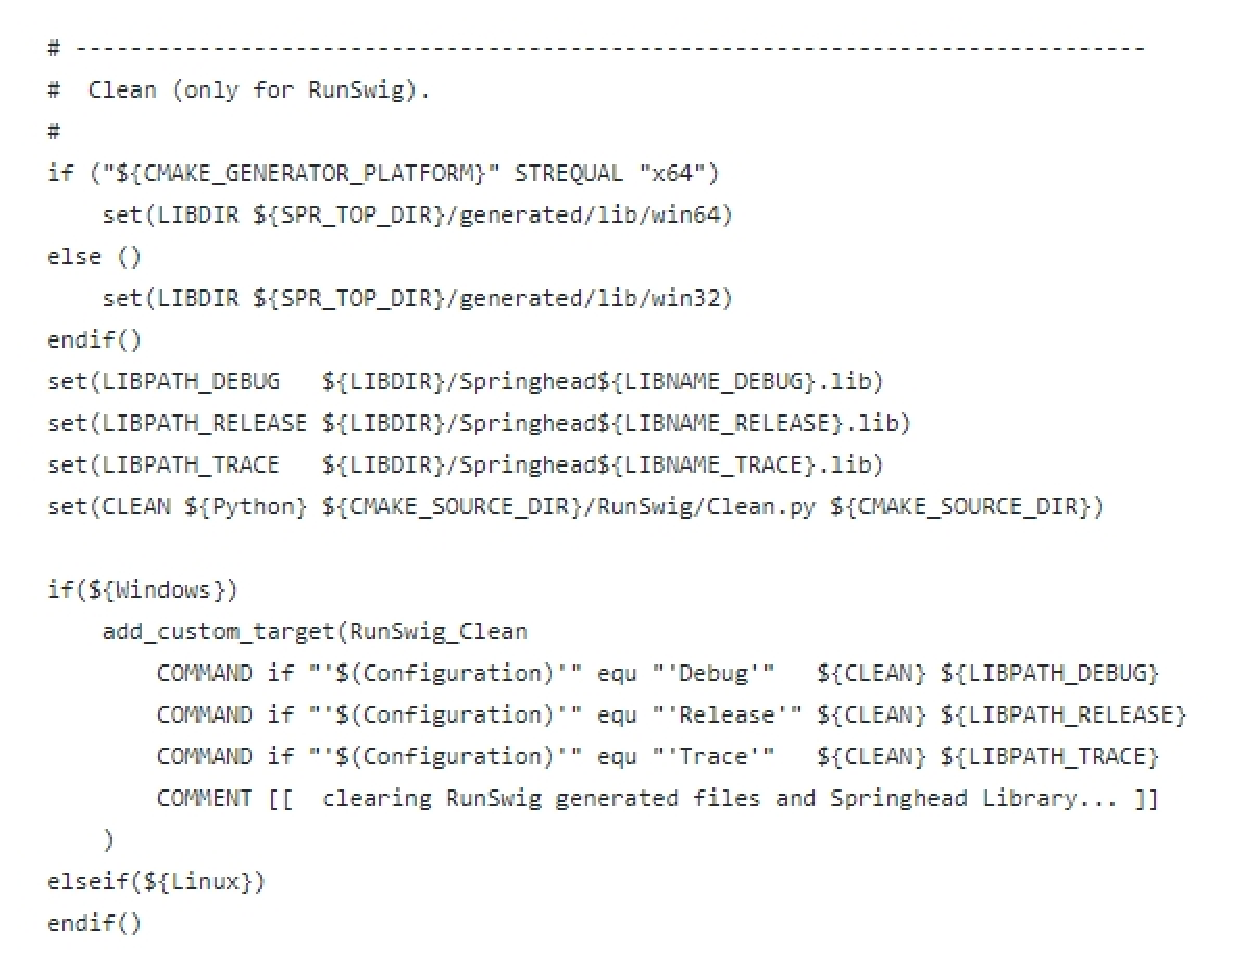
\includegraphics[width=.8\textwidth]{fig/RemoveRunSwigClean.eps}
		}\end{center}
		\label{fig:SpringheadLibraryTree}
	    \end{narrow}
	\end{figure}\end{narrow}
	
	EmbPython\_RunSwig\_Clean\KLUDGE についても同様です。	
	
\end{narrow}

% end: 3.3.BuildApplication.tex

% ---------------------------

\end{document}
% end: main.tex
